\section{Intermediate Representation}

Intermediate representation (IR) adalah representasi internal program yang berada di antara bahasa sumber dan kode mesin target. Secara formal, IR dapat didefinisikan sebagai struktur data atau bahasa perantara yang menyimpan semantik program secara lengkap namun independen dari sintaks bahasa sumber maupun arsitektur mesin target \cite{aho2007compilers,cooper2011engineering}. Keberadaan IR memungkinkan pemisahan yang jelas antara frontend dan backend compiler.

Dalam taksonomi compiler, IR diklasifikasikan berdasarkan kedekatannya dengan sumber atau mesin. High-level IR mempertahankan struktur kontrol dan tipe data tingkat tinggi sehingga cocok untuk optimasi berbasis sumber, seperti eliminasi subekspresi umum. Low-level IR mendekati bahasa mesin dengan register tak terbatas atau memori eksplisit sehingga memudahkan alokasi register dan penjadwalan instruksi. Beberapa bentuk IR yang dikenal dalam literatur adalah Three-Address Code (TAC), Static Single Assignment (SSA), bytecode (misalnya JVM), dan P-code yang dikembangkan oleh Wirth untuk mesin stack \cite{appel1998modern,wirth1976algorithms}.

Ada tiga alasan fundamental mengapa compiler modern menggunakan IR. Pertama, \textit{machine independence}: frontend compiler tidak perlu mengetahui arsitektur target karena hasil analisis disimpan dalam IR. Kedua, \textit{optimization opportunity}: IR menyediakan level abstraksi yang lebih mudah dianalisis dan dioptimasi dibandingkan source code atau kode mesin. Ketiga, \textit{portability}: dengan IR yang sama, satu frontend dapat dipasangkan dengan banyak backend untuk mesin berbeda, dan sebaliknya satu backend dapat melayani banyak bahasa sumber.

\begin{figure}[H]
    \centering
    \begin{tikzpicture}[
        scale=0.90,
        transform shape,
        node distance=8mm and 12mm,
        every node/.style={draw, rounded corners, align=center, minimum width=2.6cm, minimum height=7mm, font=\small},
        arrow/.style={-{Stealth[length=2.5mm]}, thick}
        ]
        \node (src) {Source Code};
        \node (lex) [below=of src] {Lexer};
        \node (tok) [below=of lex] {Token Stream};
        \node (par) [below=of tok] {Parser};
        \node (pt) [below=of par] {Parse Tree};
        \node (astb) [below=of pt] {AST Builder};
        \node (ast) [below=of astb] {AST};
        \node (sem) [below=of ast] {Semantic Analyzer};
        \node (da) [below=of sem] {Decorated AST};
        \node (ir) [below=of da] {IR / TAC};
        \node (opt) [right=of ir] {Optimizer};
        \node (cg) [below=of ir] {Code Gen};
        \node (vm) [below=of cg] {VM / Interpreter};

        \draw[arrow] (src) -- (lex);
        \draw[arrow] (lex) -- (tok);
        \draw[arrow] (tok) -- (par);
        \draw[arrow] (par) -- (pt);
        \draw[arrow] (pt) -- (astb);
        \draw[arrow] (astb) -- (ast);
        \draw[arrow] (ast) -- (sem);
        \draw[arrow] (sem) -- (da);
        \draw[arrow] (da) -- (ir);
        \draw[arrow] (ir) -- (opt);
        \draw[arrow] (opt) -- (cg);
        \draw[arrow] (ir) -- (cg);
        \draw[arrow] (cg) -- (vm);
    \end{tikzpicture}
    \caption{Pipeline compiler lengkap dari source code hingga eksekusi mesin virtual}
    \label{fig:intermediate-pipeline}
\end{figure}

Gambar \ref{fig:intermediate-pipeline} menunjukkan pipeline compiler lengkap mulai dari source code hingga eksekusi oleh mesin virtual. Frontend meliputi lexer, parser, AST builder, dan semantic analyzer yang menghasilkan decorated AST. Backend dimulai dari intermediate code generator yang meratakan decorated AST menjadi IR berupa TAC. IR tersebut dapat dioptimasi sebelum diterjemahkan ke kode mesin target oleh code generator, atau dieksekusi langsung oleh virtual machine interpreter.


\section{Three-Address Code}

Three-Address Code (TAC) adalah format IR yang setiap instruksinya melibatkan maksimal tiga alamat: dua operand sumber dan satu lokasi tujuan \cite{aho2007compilers}. Dalam konteks TAC, \textit{address} tidak selalu berupa alamat memori fisik, melainkan dapat berupa nama variabel, konstanta literal, atau variabel sementara yang dihasilkan compiler \cite{cooper2011engineering}. Variabel sementara ini biasanya dinamai \texttt{t1}, \texttt{t2}, \texttt{t3}, dan seterusnya, sesuai dengan urutan pembuatannya selama traversal ekspresi.

Pembentukan TAC dari ekspresi kompleks dilakukan melalui traversal \textit{post-order} pada pohon ekspresi. Setiap node internal diterjemahkan menjadi satu instruksi TAC, sedangkan daun-daunnya menjadi operand. Sebagai contoh, ekspresi \texttt{x := (a + b) * (c - d)} menghasilkan empat instruksi TAC berikut.

\begin{tcolorbox}[title=Contoh TAC,colback=gray!5,colframe=black!60,boxrule=0.5pt,arc=2mm]
\begin{verbatim}
t1 := a + b
t2 := c - d
t3 := t1 * t2
x  := t3
\end{verbatim}
\end{tcolorbox}

Nama variabel sementara umumnya mengikuti konvensi \texttt{t} yang diikuti nomor urut. Compiler dapat menggunakan berbagai strategi penamaan, namun yang paling penting adalah keunikan nama dalam satu prosedur dan tidak bertabrakan dengan nama variabel program. Setelah nilai variabel sementara tidak lagi dibutuhkan, nama tersebut dapat \textit{reuse}. Analisis \textit{liveness} digunakan untuk menentukan kapan variabel sementara masih \textit{hidup} (masih akan digunakan di masa depan) dan kapan sudah \textit{mati} (tidak akan digunakan lagi). Variabel yang sudah mati dapat di-assign ulang ke ekspresi baru tanpa kehilangan informasi.

Dalam literatur compiler, TAC direpresentasikan dalam tiga bentuk utama: \textit{quadruples}, \textit{triples}, dan \textit{indirect triples} \cite{aho2007compilers}. Quadruples menyimpan setiap instruksi sebagai tupel empat elemen (op, arg1, arg2, result), sehingga setiap instruksi dapat diacu secara eksplisit. Triples menyimpan tiga elemen (op, arg1, arg2) dengan hasil implisit berupa indeks instruksi itu sendiri, yang mengurangi ruang penyimpanan namun mempersulit pemindahan kode. Indirect triples menambahkan tabel pointer ke triples, sehingga memungkinkan penyusunan ulang instruksi tanpa mengubah isi triples. Tabel \ref{tab:tac-repr} membandingkan ketiga representasi untuk ekspresi \texttt{x = a + b * c}.

\begin{table}[H]
    \centering
    \caption{Perbandingan representasi TAC}
    \label{tab:tac-repr}
    \small
    \begin{tabularx}{\textwidth}{c X X X}
        \toprule
        \textbf{No} & \textbf{Quadruples} & \textbf{Triples} & \textbf{Indirect Triples} \\
        \midrule
        0 & (MUL, b, c, t1) & (0) MUL b c & (0) $\rightarrow$ 100 \\
        1 & (ADD, a, t1, t2) & (1) ADD a (0) & (1) $\rightarrow$ 101 \\
        2 & (ASSIGN, t2, \_, x) & (2) ASSIGN x (1) & (2) $\rightarrow$ 102 \\
        \bottomrule
    \end{tabularx}
\end{table}


\section{Stack Machine dan Instruction Set Architecture}

Arsitektur mesin eksekusi untuk intermediate code dapat diklasifikasikan menjadi tiga paradigma utama: \textit{stack machine}, \textit{register machine}, dan \textit{accumulator machine}. Stack machine menggunakan struktur stack implisit sebagai tempat operan; setiap instruksi mempop operand dari stack, melakukan operasi, dan mempush hasilnya kembali \cite{wirth1976algorithms}. Register machine menggunakan register eksplisit sebagai operand (misalnya x86, ARM), sedangkan accumulator machine hanya memiliki satu register implisit sebagai akumulator. Stack machine dipilih secara luas pada compiler edukasional karena format instruksinya sangat sederhana dan codegen dari AST menjadi sangat langsung.

Salah satu contoh klasik stack machine adalah P-code machine yang dikembangkan Niklaus Wirth untuk compiler Pascal. P-code menggunakan instruksi berbasis stack dengan format tiga field: opcode, level leksikal, dan operand \cite{wirth1976algorithms}. Level leksikal merepresentasikan kedalaman \textit{static scoping}, sedangkan operand menyimpan nilai literal, offset memori, atau alamat instruksi. Mekanisme ini memungkinkan akses variabel non-lokal melalui traversal \textit{static link chain}.

Konsep \textit{lexical addressing} menjadi fondasi akses variabel dalam bahasa dengan \textit{static scoping}. Setiap variabel diakses melalui pasangan \texttt{(level, offset)}, di mana level menunjukkan jarak leksikal dari variabel terhadap scope saat ini, dan offset menunjukkan posisi relatif dalam frame memori. Static scoping berbeda dengan dynamic scoping: pada static scoping, ruang lingkup variabel ditentukan oleh struktur tekstual program (letak deklarasi), sedangkan pada dynamic scoping ditentukan oleh urutan pemanggilan fungsi pada runtime. Compiler modern hampir selalu menggunakan static scoping karena lebih mudah dianalisis dan diprediksi.

Fungsi standar untuk menelusuri static link dalam interpreter stack machine adalah \texttt{base(l, b)}, yang secara rekursif mengikuti static link sebanyak $l$ level dari base pointer $b$ saat ini. Fungsi ini didefinisikan sebagai berikut.

\begin{breakablealgorithm}[Fungsi base untuk Static Link Traversal]
    \label{alg:base-func}
    \begin{algorithmic}[1]
        \Function{base}{$l$, $b$}
        \While{$l > 0$}
            \State $b \gets \text{stack}[b]$ \Comment{static link ada di slot 0}
            \State $l \gets l - 1$
        \EndWhile
        \State \Return $b$
        \EndFunction
    \end{algorithmic}
\end{breakablealgorithm}

Pada saat eksekusi, instruksi \texttt{LOD l a} (load) dan \texttt{STO l a} (store) menggunakan fungsi \texttt{base(l, b)} untuk menemukan base pointer frame yang tepat sebelum mengakses slot offset \texttt{a}. Jika \texttt{l = 0}, variabel berada pada frame saat ini sehingga tidak perlu traversal. Jika \texttt{l > 0}, interpreter mengikuti static link chain sebanyak \texttt{l} level, yang memungkinkan prosedur bersarang untuk mengakses variabel dari scope induk secara leksikal.


\section{Activation Record dan Stack Frame}

\textit{Activation record}, atau \textit{stack frame}, adalah blok memori kontigu yang dibuat setiap kali sebuah prosedur dipanggil. Blok ini menyimpan seluruh konteks eksekusi prosedur tersebut, termasuk variabel lokal, argumen, alamat pengembalian, serta tautan ke frame lain \cite{aho2007compilers}. Stack frame bekerja dengan prinsip LIFO (Last In, First Out): frame baru di-push ke pucuk stack saat pemanggilan, dan di-pop saat prosedur selesai, sehingga seluruh variabel lokalnya otomatis musnah.

Setiap stack frame memiliki tiga slot header wajib. \textbf{Static link} (slot 0) menunjuk ke base pointer frame induk secara leksikal berdasarkan kedalaman \textit{static scoping}. \textbf{Dynamic link} (slot 1) menunjuk ke base pointer frame pemanggil pada runtime. \textbf{Return address} (slot 2) menyimpan indeks instruksi yang harus dieksekusi setelah prosedur selesai. Slot-slot setelah header digunakan untuk parameter, variabel lokal, dan operand sementara selama evaluasi ekspresi.

\begin{figure}[H]
    \centering
    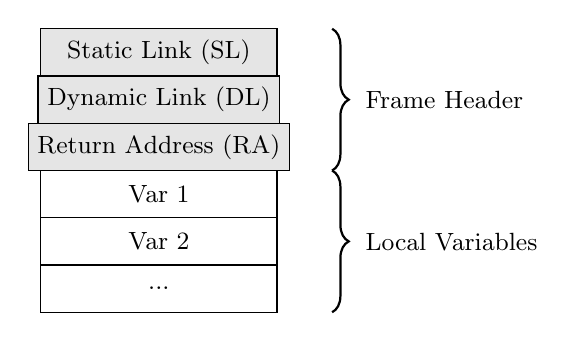
\begin{tikzpicture}[
        box/.style={draw, minimum width=3cm, minimum height=0.6cm, font=\small},
        label/.style={font=\small}
    ]
        \node[box, fill=gray!20] (sl) at (0,3) {Static Link (SL)};
        \node[box, fill=gray!20] (dl) at (0,2.4) {Dynamic Link (DL)};
        \node[box, fill=gray!20] (ra) at (0,1.8) {Return Address (RA)};
        \node[box] (v1) at (0,1.2) {Var 1};
        \node[box] (v2) at (0,0.6) {Var 2};
        \node[box] (v3) at (0,0) {...};
        \draw[decorate,decoration={brace,amplitude=6pt},thick] (2.2,3.3) -- (2.2,1.5);
        \node[label,right] at (2.5,2.4) {Frame Header};
        \draw[decorate,decoration={brace,amplitude=6pt},thick] (2.2,1.5) -- (2.2,-0.3);
        \node[label,right] at (2.5,0.6) {Local Variables};
    \end{tikzpicture}
    \caption{Ilustrasi stack frame dengan static link, dynamic link, dan return address}
    \label{fig:stack-frame}
\end{figure}

Pemilihan stack sebagai struktur memori eksekusi didasarkan pada kebutuhan scope dan pemanggilan prosedur. Array biasa tidak dapat secara otomatis mengelola siklus hidup variabel lokal karena tidak memiliki mekanisme push-pop yang terkait dengan aktivasi dan deaktivasi prosedur.


\section{Translasi Control Flow dan Backpatching}

Penerjemahan struktur kontrol seperti percabangan dan perulangan ke dalam IR memerlukan teknik \textit{syntax-directed translation} (SDT). SDT adalah metode code generation yang menggunakan atribut pada node pohon sintaks untuk membimbing pembentukan instruksi \cite{aho2007compilers}. Atribut \textit{synthesized} mengalir dari anak ke induk (misalnya fragmen kode yang dihasilkan oleh subekspresi), sedangkan atribut \textit{inherited} mengalir dari induk ke anak (misalnya label berikutnya yang harus dituju setelah suatu blok).

Tantangan utama dalam translasi control flow adalah penanganan instruksi lompatan yang belum mengetahui targetnya pada saat instruksi tersebut dihasilkan. Solusinya adalah teknik \textit{backpatching}. Secara formal, backpatching bekerja dengan memelihara \textit{backpatch list}, yaitu himpunan indeks instruksi yang memiliki target lompatan kosong. Tiga operasi fundamental didefinisikan: \texttt{backpatch(L, i)} mengisi semua indeks dalam list $L$ dengan target $i$; \texttt{merge(L1, L2)} menggabungkan dua backpatch list; dan \texttt{makelist(i)} membuat list baru berisi indeks tunggal $i$ \cite{aho2007compilers}.

Sebagai contoh, translasi \texttt{if-then-else} menggunakan dua backpatch list. List \texttt{falses} menyimpan indeks \texttt{JPC} yang melompat ke blok \texttt{else}, sedangkan list \texttt{nexts} menyimpan indeks \texttt{JMP} yang melompat ke akhir percabangan. Setelah posisi label \texttt{else} diketahui, \texttt{falses} di-backpatch. Setelah posisi label akhir diketahui, \texttt{nexts} di-backpatch.

\begin{tcolorbox}[title=Contoh TAC untuk IF-ELSE dengan Backpatching,colback=gray!5,colframe=black!60,boxrule=0.5pt,arc=2mm]
\begin{verbatim}
{ evaluasi kondisi }
JPC 0 _        // falses = makelist(ip)
{ blok then }
JMP 0 _        // nexts = makelist(ip)
L_ELSE:
{ blok else }
L_END:
backpatch(falses, L_ELSE)
backpatch(nexts, L_END)
\end{verbatim}
\end{tcolorbox}

Perulangan \texttt{while} menggunakan pola yang sama. Label \texttt{L\_START} dipasang sebelum evaluasi kondisi. Instruksi \texttt{JPC} keluar ke \texttt{L\_END} yang belum diketahui, sehingga indeksnya masuk ke backpatch list. Setelah body selesai, \texttt{JMP} kembali ke \texttt{L\_START}. Label \texttt{L\_END} dipasang setelah body, lalu backpatch list diisi.

\begin{tcolorbox}[title=Contoh TAC untuk WHILE,colback=gray!5,colframe=black!60,boxrule=0.5pt,arc=2mm]
\begin{verbatim}
L_START:
{ evaluasi kondisi }
JPC 0 _        // exits = makelist(ip)
{ blok body }
JMP 0 L_START
L_END:
backpatch(exits, L_END)
\end{verbatim}
\end{tcolorbox}

Perulangan \texttt{repeat-until} memiliki karakteristik berbeda karena body selalu dieksekusi setidaknya sekali. Body diterjemahkan terlebih dahulu, kemudian kondisi dievaluasi. Jika kondisi bernilai salah (belum terpenuhi), \texttt{JPC} melompat kembali ke awal body menggunakan backpatch list.

\begin{tcolorbox}[title=Contoh TAC untuk REPEAT-UNTIL,colback=gray!5,colframe=black!60,boxrule=0.5pt,arc=2mm]
\begin{verbatim}
L_START:
{ blok body }
{ evaluasi kondisi }
JPC 0 _        // repeats = makelist(ip)
L_END:
backpatch(repeats, L_START)
\end{verbatim}
\end{tcolorbox}

Translasi \texttt{for} dan \texttt{case} juga bergantung pada backpatching. For loop memerlukan backpatching untuk lompatan keluar dari loop, sedangkan case statement memerlukan backpatching untuk setiap branch agar tidak jatuh secara implisit ke branch berikutnya (\textit{fall-through}).


\section{Runtime Vulnerabilities}

Interpreter yang mengeksekusi IR beroperasi pada level yang lebih dekat dengan mesin dibandingkan bahasa sumber, sehingga rentan terhadap kerentanan yang berkaitan dengan manajemen memori dan alur eksekusi. \textit{Memory safety} dalam konteks stack machine mencakup dua aspek: \textit{spatial safety} (memastikan setiap akses memori berada dalam batas yang valid) dan \textit{temporal safety} (memastikan memori tidak diakses setelah dilepaskan) \cite{aho2007compilers}.

\subsection{Kerentanan pada Stack}

\textbf{Stack overflow} terjadi ketika kedalaman pemanggilan prosedur melampaui kapasitas maksimum stack yang dialokasikan. Kondisi ini paling umum disebabkan oleh rekursi tak terbatas, di mana sebuah fungsi terus memanggil dirinya sendiri tanpa kondisi berhenti. Dampaknya adalah interpreter kehabisan memori untuk menyimpan frame baru, yang pada akhirnya menyebabkan program crash atau hang. Sebagai contoh, prosedur \texttt{recur} yang memanggil dirinya sendiri secara langsung akan menghasilkan error \texttt{stack overflow} setelah kedalaman frame melebihi batas yang ditetapkan.

\textbf{Stack underflow} merupakan kondisi inverse, yaitu ketika interpreter diinstruksikan untuk mengambil nilai dari stack operand yang sudah sepenuhnya kosong. Hal ini biasanya menandakan adanya cacat logika pada intermediate code generator, misalnya ketika sebuah operasi biner hanya memiliki satu operand di stack. Dampaknya adalah interpreter membaca nilai sampah atau memori yang tidak valid, yang dapat merusak seluruh komputasi selanjutnya.

\textbf{Stack smashing} adalah bentuk klasik dari buffer overflow pada stack machine. Dalam arsitektur ini, frame header (static link, dynamic link, dan return address) diletakkan secara bersebelahan dengan variabel lokal. Jika interpreter mengizinkan penulisan data melebihi ukuran variabel lokalnya, data tersebut dapat meluber dan menimpa return address. Akibatnya, saat prosedur selesai dieksekusi, interpreter akan melompat ke alamat memori yang salah, yang berpotensi mengeksekusi kode berbahaya atau menyebabkan crash sistem.

Pendekatan umum untuk menangani ketiga kerentanan stack adalah dengan menambahkan validasi sebelum setiap operasi yang berpotensi berbahaya. Sebelum membuat frame baru melalui instruksi \texttt{CAL}, interpreter harus memeriksa apakah kedalaman stack saat ini masih di bawah batas maksimum. Sebelum melakukan operasi \texttt{pop}, interpreter harus memastikan bahwa stack pointer masih berada di atas base pointer frame saat ini ditambah ukuran header. Sebelum menulis ke memori melalui \texttt{STO}, interpreter harus memverifikasi bahwa slot target bukan merupakan slot header yang dilindungi. Algoritma berikut mengilustrasikan validasi yang dilakukan sebelum pembuatan frame baru.

\begin{breakablealgorithm}[Validasi Sebelum Pembuatan Frame Baru]
    \label{alg:stack-validation}
    \begin{algorithmic}[1]
        \Procedure{validatePushFrame}{}
        \If{$\text{currentDepth} \geq \text{kMaxStackFrames}$}
            \State \textbf{error} \texttt{stack overflow}
        \EndIf
        \EndProcedure
    \end{algorithmic}
\end{breakablealgorithm}

\subsection{Kerentanan Memori dan Akses: Out-of-Bounds Variable Access}

\textbf{Out-of-bounds variable access} adalah kerentanan yang terjadi ketika program mencoba mengakses indeks array di luar batas yang dideklarasikan. Dalam konteks stack machine, setiap elemen array dialokasikan secara kontigu di dalam stack frame. Jika interpreter mengizinkan akses indeks melebihi batas atas atau kurang dari batas bawah, maka akses tersebut akan mengarah ke memori milik variabel lain atau bahkan frame header, yang melanggar \textit{spatial safety}.

Dampak dari kerentanan ini dapat sangat serius. Penulisan ke indeks yang salah dapat merusak nilai variabel lain secara diam-diam, yang menyebabkan bug yang sulit dilacak. Dalam kasus ekstrem, penulisan tersebut dapat menimpa return address dan memicu stack smashing. Sebagai contoh, jika sebuah array dideklarasikan dengan batas \texttt{array[1..3]}, namun program mencoba mengakses \texttt{array[5]}, maka interpreter harus mencegat akses tersebut sebelum mencapai memori fisik.

Pendekatan umum untuk menangani kerentanan ini adalah dengan melakukan \textit{bounds checking} pada setiap operasi akses array. Interpreter membandingkan indeks yang diminta dengan batas bawah (\texttt{low}) dan batas atas (\texttt{high}) yang tersimpan dalam metadata array. Jika indeks berada di luar rentang tersebut, interpreter menghentikan eksekusi dan melaporkan \texttt{IndexOutOfBoundsException}. Metadata array pada Arion disimpan dalam operand instruksi \texttt{ALOD} dan \texttt{ASTO}, yang berisi base offset, jumlah dimensi, batas rendah, dan batas tinggi untuk setiap dimensi.

\begin{tcolorbox}[title=Contoh Bounds Checking pada Array Access,colback=gray!5,colframe=black!60,boxrule=0.5pt,arc=2mm]
\begin{verbatim}
if index < low || index > high then
    error: IndexOutOfBoundsException
else
    address = base + (index - low)
    access memory at address
end
\end{verbatim}
\end{tcolorbox}

\subsection{Kerentanan Alur Eksekusi: Invalid Jump Targets}

\textbf{Invalid jump targets} terjadi ketika intermediate code generator menghasilkan instruksi lompatan (\texttt{JMP}, \texttt{JPC}, atau \texttt{CAL}) yang menuju ke alamat instruksi yang tidak pernah ada dalam daftar program. Kondisi ini dapat disebabkan oleh kesalahan pada mekanisme backpatching, di mana alamat target tidak diisi dengan benar setelah seluruh instruksi dihasilkan. Dampaknya adalah instruction pointer (IP) akan melompat ke luar batas vektor instruksi, yang menyebabkan interpreter membaca memori yang tidak valid dan crash secara tiba-tiba.

Sebagai contoh, jika sebuah program memiliki 20 instruksi (indeks 0 hingga 19), namun instruksi ke-5 berisi \texttt{JMP 0 25}, maka lompatan tersebut akan mengarah ke alamat yang tidak pernah didefinisikan. Tanpa validasi, interpreter akan mencoba membaca instruksi ke-25 dan menghasilkan perilaku tak terdefinisi.

Pendekatan umum untuk menangani kerentanan ini adalah dengan melakukan \textit{pre-execution validation} terhadap seluruh target lompatan sebelum siklus fetch-decode-execute dimulai. Interpreter melakukan satu kali traversal pada seluruh daftar instruksi untuk mengumpulkan semua alamat target yang direferensi oleh instruksi lompatan. Kemudian, setiap target tersebut diverifikasi agar berada dalam rentang valid (0 hingga program.size() - 1). Jika ada target yang tidak valid, interpreter langsung menghentikan eksekusi dan melaporkan \texttt{InvalidJumpTargetException} tanpa mengeksekusi satu instruksi pun. Strategi ini lebih aman karena mencegah state mesin menjadi korup sejak awal.

\begin{breakablealgorithm}[Validasi Target Jump Sebelum Eksekusi]
    \label{alg:jump-validation}
    \begin{algorithmic}[1]
        \Procedure{validateJumpTargets}{program}
        \For{each inst in program}
            \If{inst.opcode \textbf{in} \{JMP, JPC, CAL\}}
                \If{inst.operand $<$ 0 \textbf{or} inst.operand $\geq$ program.size()}
                    \State \textbf{error} \texttt{InvalidJumpTargetException}
                \EndIf
            \EndIf
        \EndFor
        \EndProcedure
    \end{algorithmic}
\end{breakablealgorithm}

\subsection{Kerentanan Aritmatika: Numerical Overflow/Underflow}

\textbf{Numerical overflow} terjadi ketika hasil operasi aritmatika melebihi nilai maksimum yang dapat ditampung oleh tipe data integer, sedangkan \textbf{numerical underflow} terjadi ketika hasil operasi jatuh di bawah nilai minimum. Dalam representasi signed integer 32-bit, nilai maksimum adalah sekitar 2.147.483.647 dan nilai minimum adalah sekitar -2.147.483.648. Jika sebuah operasi penjumlahan menghasilkan nilai di luar rentang tersebut, maka akan terjadi \textit{wrap-around}, di mana nilai positif besar tiba-tiba menjadi negatif, atau sebaliknya.

Dampak dari kerentanan ini dapat sangat merusak logika program. Sebagai contoh, sebuah perulangan yang menggunakan variabel penghitung integer dapat menjadi infinite loop jika variabel tersebut overflow dari nilai positif maksimum kembali ke nilai negatif. Dalam aplikasi finansial atau ilmiah, hasil perhitungan yang salah karena overflow dapat menghasilkan keputusan yang fatal.

Pendekatan umum untuk menangani kerentanan ini adalah dengan menggunakan \textit{checked arithmetic}. Sebelum melakukan operasi, interpreter memeriksa apakah hasil operasi akan melampaui batas tipe data. Untuk penjumlahan dua bilangan positif, interpreter memeriksa apakah \texttt{a > INT\_MAX - b}. Untuk pengurangan, interpreter memeriksa apakah \texttt{a < INT\_MIN + b}. Untuk perkalian, pemeriksaan lebih kompleks karena harus mempertimbangkan tanda kedua operand. Jika pemeriksaan menunjukkan bahwa overflow atau underflow akan terjadi, interpreter menghentikan eksekusi dan melaporkan \texttt{OverflowError} atau \texttt{UnderflowError}. Strategi ini lebih aman dibandingkan \textit{silent wrap-around} karena memberi tahu programmer bahwa ada kesalahan logika yang perlu diperbaiki.

\begin{tcolorbox}[title=Contoh Checked Addition,colback=gray!5,colframe=black!60,boxrule=0.5pt,arc=2mm]
\begin{verbatim}
function checkedAdd(a, b):
    if a > 0 and b > INT_MAX - a then
        error: OverflowError
    else if a < 0 and b < INT_MIN - a then
        error: UnderflowError
    else
        return a + b
    end
\end{verbatim}
\end{tcolorbox}
